\documentclass[a4paper]{report}
\usepackage{algorithmic}
\usepackage{array}
\usepackage{url,amsfonts,amsmath,amssymb,amsthm,color,enumerate,tikz,hyperref}
\usepackage{algorithm,bbm}
\usepackage{mathtools}
% \usepackage{indentfirst}
\usepackage{stackrel}
\usepackage{listings}
\usepackage{subfigure}
\usepackage{subfloat}
\usepackage[justification=centering]{caption}
\usepackage{booktabs} % for three-line table
% \usepackage{subfig}
\usepackage{graphicx}
\setcounter{tocdepth}{4}
\setcounter{secnumdepth}{4}

\hyphenation{op-tical net-works semi-conduc-tor}
\usetikzlibrary{shapes, shadows, arrows}
% \usepackage[english]{babel}
% \usepackage[utf8]{inputenc}
% \usepackage{amsmath}
% \usepackage{graphicx}
% \usepackage[colorinlistoftodos]{todonotes}

\title{Get Start with gr-cdma}

\author{Yu Wang\\umwangyu@umich.edu}

\date{\today}

% def some function
\DeclarePairedDelimiter\ceil{\lceil}{\rceil}
\DeclarePairedDelimiter\floor{\lfloor}{\rfloor}

\newcommand{\specialcell}[2][c]{%
  \begin{tabular}[#1]{@{}c@{}}#2\end{tabular}}

\begin{document}
\maketitle
\tableofcontents
\newpage




% \chapter{Introduction}
\section{What is gr-cdma}
Project gr-cdma is the physical layer of CDMA communication. This project is developed based on GNURadio\cite{GNURadio}.
gr-cdma is created and maintained by Prof. Anastasopoulos.
The whole source codes are on github \url{https://github.com/anastas/gr-cdma}.
This project is to build a communication block which employs DS-CDMA technique to build the link.
The user does not have to know the details of the schemes, but could transmit reliably through this physical layer protocol.

\section{What is GNURadio}
GNURadio\cite{GNURadio} is a open-source *unix based platform which enables developers and researchers design and test their self-built communication or signal processing system.
The whole platform is written by c++. Developer could use c++ or python to customize their own block. gr-cdma is a customized block as well.

\section{What is the Current State of gr-cdma}
Till 17-Jun-2016, the main part of this project is finished.
The next step is to optimize the working strategy for several block to make the system more robust in field test. 
This document is an introduction of what this project is, how to get start with GNURadio and gr-cdma and what are the issues to be solved. 
\chapter{Introduction}
\section{What is gr-cdma}
Project gr-cdma is the physical layer of CDMA communication. This project is developed based on GNURadio\cite{GNURadio}.
gr-cdma is created and maintained by Prof. Anastasopoulos.
The whole source codes are on github \url{https://github.com/anastas/gr-cdma}.
This project is to build a communication block which employs DS-CDMA technique to build the link.
The user does not have to know the details of the schemes, but could transmit reliably through this physical layer protocol.

\section{What is GNURadio}
GNURadio\cite{GNURadio} is a open-source *unix based platform which enables developers and researchers design and test their self-built communication or signal processing system.
The whole platform is written by c++. Developer could use c++ or python to customize their own block. gr-cdma is a customized block as well.

\section{What is the Current State of gr-cdma}
Till 17-Jun-2016, the main part of this project is finished.
The next step is to optimize the working strategy for several block to make the system more robust in field test. 
This document is an introduction of what this project is, how to get start with GNURadio and gr-cdma and what are the issues to be solved. 



% \chapter{Working Strategy of gr-cdma}
In this chapter, we will discuss the working strategy of gr-cdma, the principle of each main block.
Mathematic models and analyses are involved to describe the situation.

\section{The diagram of The Tx \& Rx}
Here are the digrams for Tx and Rx. 
\begin{figure}[!ht]
	\centering
	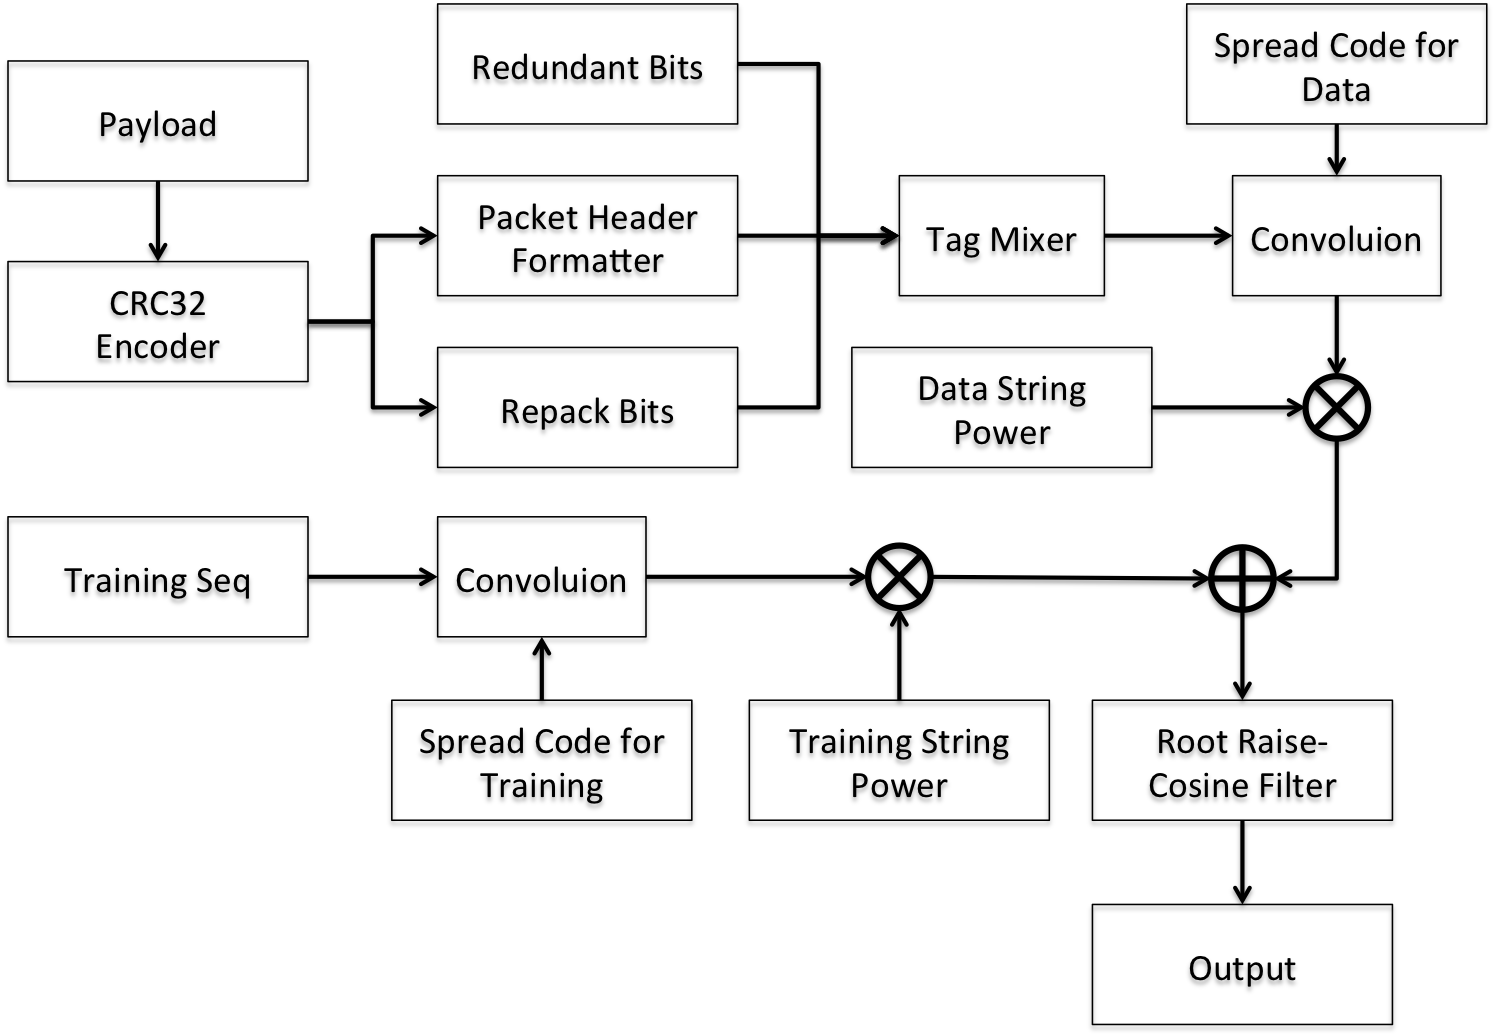
\includegraphics[width = 5 in]{figure/tx-diagram.png}
	\caption{Diagram for Tx}
	\label{fig:diagram for Tx}
\end{figure}
\begin{figure}[!ht]
	\centering
	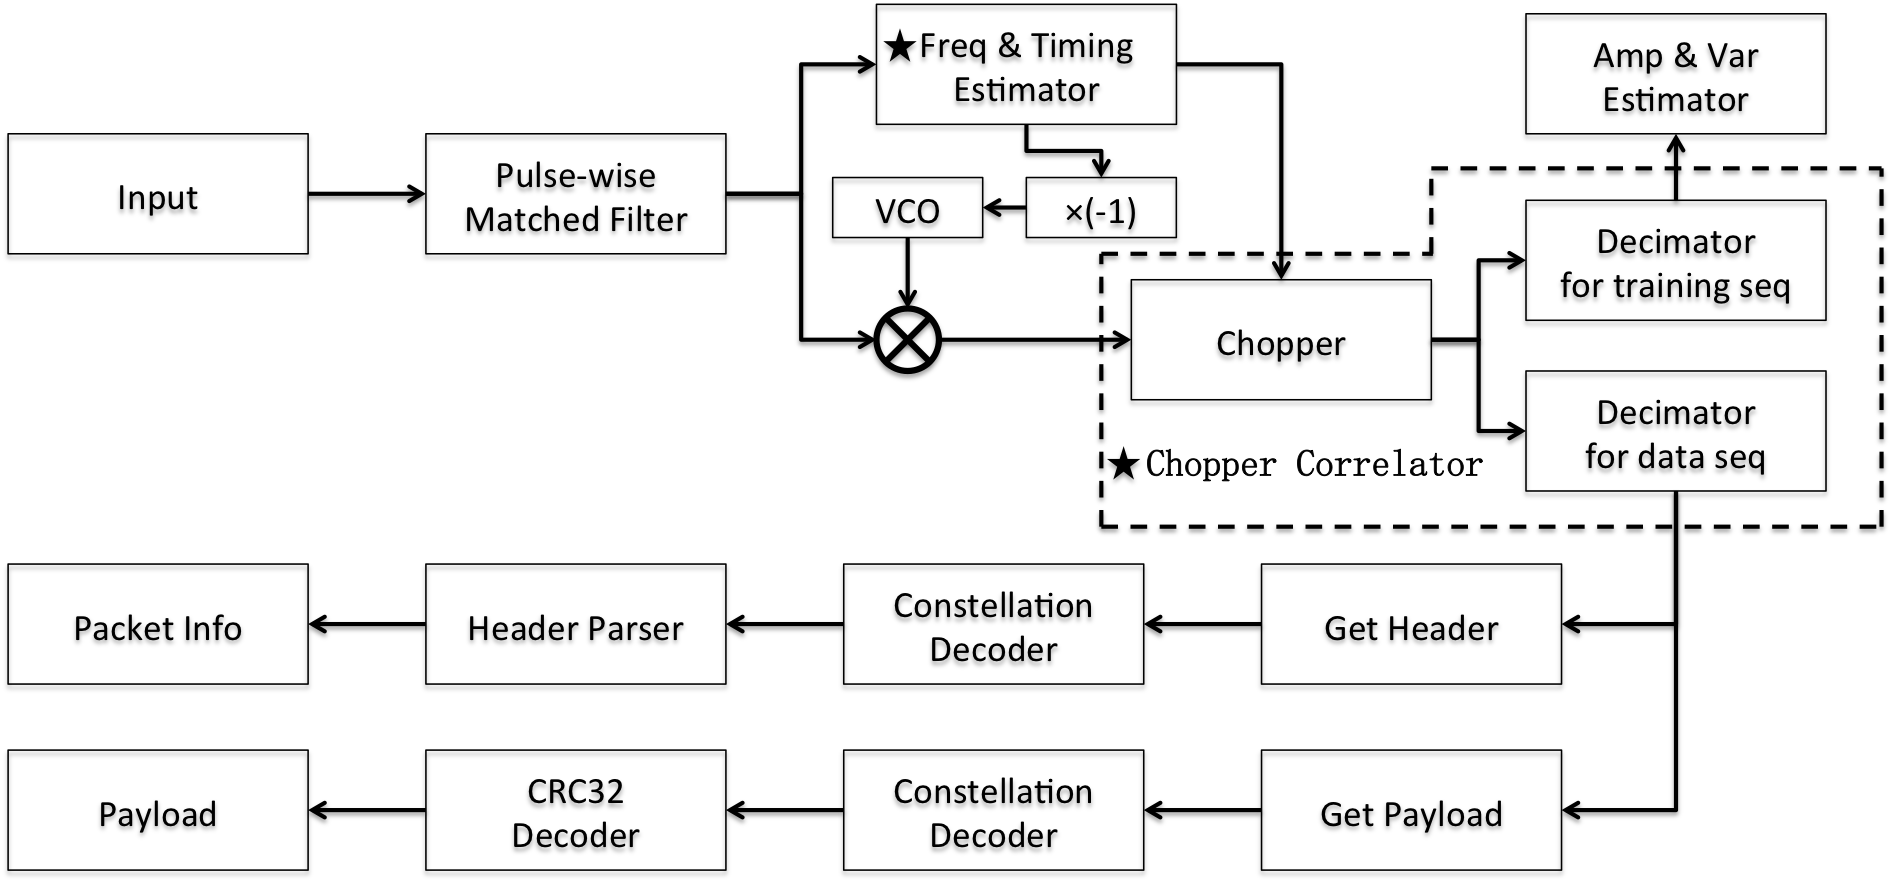
\includegraphics[width = 5in]{figure/rx-diagram.png}
	\caption{Diagram for Rx}
	\label{fig:diagram for Rx}
\end{figure}

From fig \ref{fig:diagram for Tx} and fig \ref{fig:diagram for Rx}, you may find that the system is a little bit more complicated than you thought. And also, the receiver is bigger than the transmitter. In fact, it is for the reason that the receiver will deal with no only the decoding part, but also the synchronization problem. which is actually the most difficult part for this system.

\section{Transmitter} % (fold)
\label{sec:transmitter}
The duty for transmitter is to package the payload or the input data, build the packet structure, generate the training sequence, modify the power for each section and form the waveform. Similar to other CDMA system, one of the essential part of the system is about the spreading code. The quality of the spreading code will affect greatly about the performance of synchronization parts. Intuitively, we would like to use codes like m-sequences and gold sequence, which has high auto-correlation and flat cross-correlation value.

\begin{figure}
	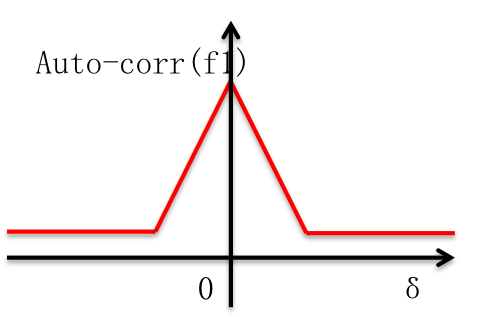
\includegraphics[width = 3in]{figure/bad_correlation.png}
	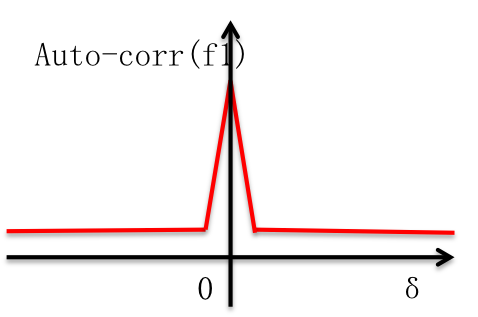
\includegraphics[width = 3in]{figure/good_correlation.png}
\end{figure}

% section transmitter (end)
\chapter{Working Strategy of gr-cdma}
In this chapter, we will discuss the working strategy of gr-cdma, the principle of each main block.
Mathematic models and analyses are involved to describe the situation.

\section{The diagram of The Tx \& Rx}
Here are the digrams for Tx and Rx. 
\begin{figure}[!ht]
	\centering
	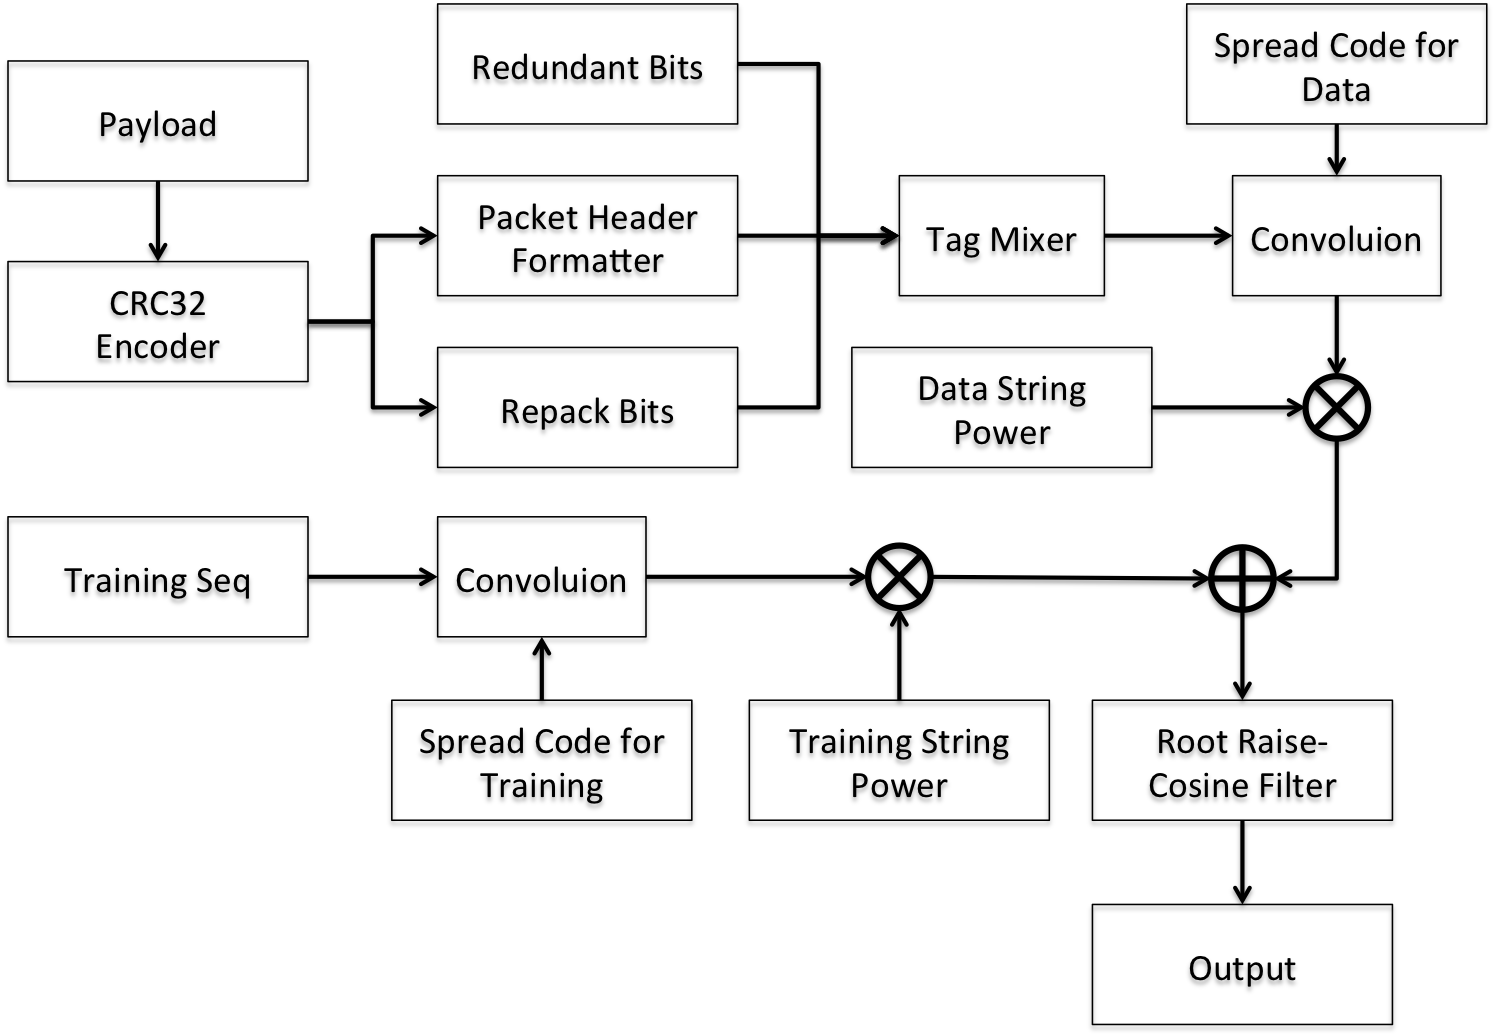
\includegraphics[width = 5 in]{figure/tx-diagram.png}
	\caption{Diagram for Tx}
	\label{fig:diagram for Tx}
\end{figure}
\begin{figure}[!ht]
	\centering
	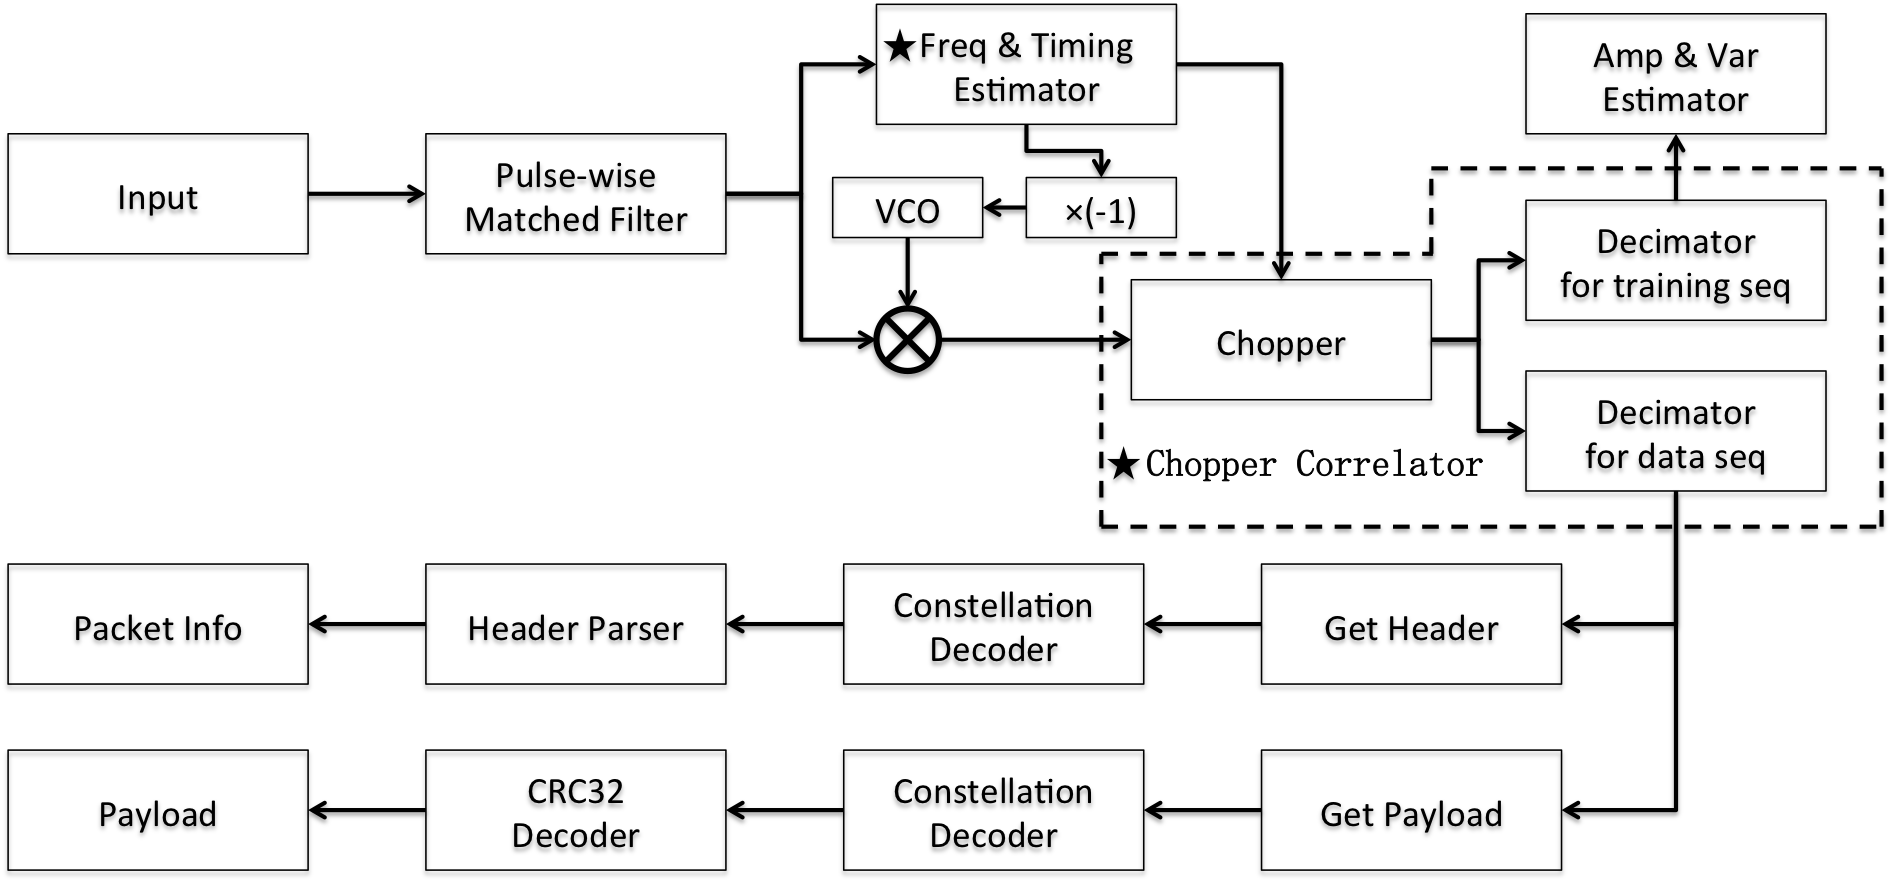
\includegraphics[width = 5in]{figure/rx-diagram.png}
	\caption{Diagram for Rx}
	\label{fig:diagram for Rx}
\end{figure}

From fig \ref{fig:diagram for Tx} and fig \ref{fig:diagram for Rx}, you may find that the system is a little bit more complicated than you thought. And also, the receiver is bigger than the transmitter. In fact, it is for the reason that the receiver will deal with no only the decoding part, but also the synchronization problem. which is actually the most difficult part for this system.

\section{Transmitter} % (fold)
\label{sec:transmitter}
The duty for transmitter is to package the payload or the input data, build the packet structure, generate the training sequence, modify the power for each section and form the waveform. 

\subsection{Spreading Code} % (fold)
\label{sub:spreading_code}

Similar to other CDMA system, one of the essential part of the system is about the spreading code. The quality of the spreading code will affect greatly about the performance of synchronization parts. Intuitively, we would like to use codes like m-sequences and gold sequence, which has high auto-correlation and flat cross-correlation value.

\begin{figure}
	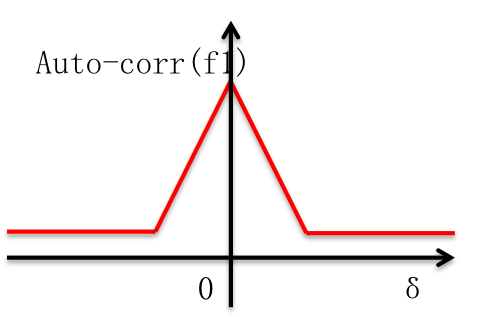
\includegraphics[width = 3in]{figure/bad_correlation.png}
	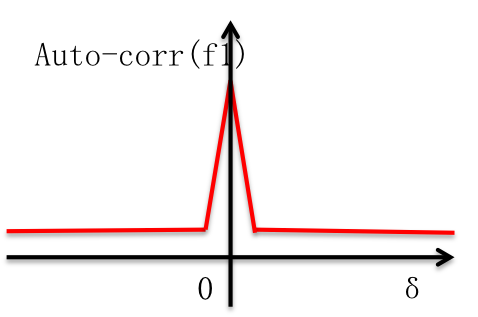
\includegraphics[width = 3in]{figure/good_correlation.png}
\end{figure}

The most famous spreading code is the m-sequence. 
\subsubsection{M-Sequence} % (fold)
\label{ssub:m_sequence}

M-sequence is a kind of sequnece with very good property. for m-sequnece $p(k)$, 
\begin{align}
	p(k) \ast p(k+\delta_k) = 
	\begin{cases}
	m    & \delta_k = 0\\
	-1	 & \delta_k \neq 0
	\end{cases}
\end{align}
$m$ is the length of sequence, $\delta_k$ ranges from $-m+1$ to $m-1$.

Here is the table for some m-sequence, table \ref{tab:M-sequence feedback connections generated using LFSR generator}

\begin{table}[ht]
\centering
\caption{M-sequence feedback connections generated using LFSR generator}
\label{tab:M-sequence feedback connections generated using LFSR generator}
\begin{tabular}{cccc}
\hline
\begin{tabular}[c]{@{}l@{}}Number \\ of shift \\ registers,\\  $L$\end{tabular} & \begin{tabular}[c]{@{}l@{}}Code \\ length \\ $N_c = 2^l-1$\end{tabular} & Feedback Taps for M-sequence & \begin{tabular}[c]{@{}l@{}}No. of \\ M-sequence \\ codes\end{tabular} \\ \hline
2 & 3 & {[}2,1{]} & 1 \\ 
3 & 7 & {[}3,2{]} & 2 \\ 
4 & 15 & {[}4,1{]} & 2 \\ 
5 & 31 & {[}5,3{]}, {[}5,4,3,2{]}, {[}5,4,2,1{]} & 6 \\ 
6 & 63 & {[}6,1{]}, {[}6,5,2,1{]}, {[}6,5,3,2{]} & 6 \\ 
7 & 127 & \begin{tabular}[c]{@{}l@{}}{[}7,1{]}, {[}7,3{]},{[}7,3,2,1{]}, {[}7,4,3,2{]}, {[}7,6,4,2{]}, \\ {[}7,6,3,1{]}, {[}7,6,5,2{]}, {[}7,6,5,4,2,1{]}, \\ {[}7,5,4,3,2,1{]}\end{tabular} & 18 \\ 
8 & 255 & \begin{tabular}[c]{@{}l@{}}{[}8,4,3,2{]}, {[}8,6,5,3{]}, {[}8,6,5,2{]}, {[}8,5,3,1{]}, \\ {[}8,6,5,1{]}, {[}8,7,6,1{]}, {[}8,7,6,5,2,1{]}, \\ {[}8,6,4,3,2,1{]}\end{tabular} & 16 \\ 
9 & 511 & \begin{tabular}[c]{@{}l@{}}{[}9,4{]}, {[}9,6,4,3{]}, {[}9,8,5,4{]}, {[}9,8,4,1{]}, \\ {[}9,5,3,2{]}, {[}9,8,6,5{]}, {[}9,8,7,2{]}, \\ {[}9,6,5,4,2,1{]}, {[}9,7,5,3,1{]}, {[}9,8,7,6,5,3{]}\end{tabular} & 48 \\ 
10 & 1023 & \begin{tabular}[c]{@{}l@{}}{[}10,3{]}, {[}10,8,3,2{]}, {[}10,4,3,1{]}, {[}10,8,5,1{]}, \\ {[}10,8,5,4{]}, {[}10,9,4,1{]}, {[}10,8,4,3{]}, \\ {[}10,5,3,2{]}, {[}10,5,2,1{]}, {[}10,9,4,2{]}, \\ {[}10,6,5,3,2,1{]}, {[}10,9,8,6,3,2{]}, \\ {[}10,9,8,7,6,5,4,3{]}, {[}10,8,7,6,5,4,3,1{]}\end{tabular} & 176 \\ \hline
\end{tabular}
\end{table}

% subsection m_sequence (end)
\subsection{Gold Sequence} % (fold)
\label{sub:gold_sequence}

But also as shown in the table above, the number of m-sequence for certain length is not that much. So, some other sequences like ``Gold sequences'' are generated. ``Gold sequence'' is actually the shift-add of two m-sequence. When the shift space for tow m-sequence is different, more relatively good sequences are generated.

% subsubsection gold_sequence (end)

\subsubsection{Spreading Seuquence used in gr-cdma} % (fold)
\label{ssub:short_seuquence}

But for gr-cdma, we adopt sequence of length 8. From the diagram, we know that a functioning system needs two spreading sequences for ``Training'' and ``Data''. So we only need two relatively good sequences. Because the length of codes are not long enough, so brutal search is feasible. 
For current system, the two sequences are as shown in table \ref{tab:Spread Codes for gr-cdma}

\begin{table}[ht]
 	\centering
 	\caption{Spread Codes for gr-cdma}
 	\label{tab:Spread Codes for gr-cdma}
 	\begin{tabular}{cc}
 	\hline
 		Type of Sequence 	& 	Sequence \\ \hline
 		Training Sequence 	& 	[+1, +1, +1, +1, -1, +1, +1, -1]\\ 
 		Data Sequence 		& 	[-1, +1, -1, +1, -1, -1, -1, -1]\\ \hline
 	\end{tabular}
 \end{table} 
% subsubsection short_seuquence (end)

% subsection spreading_code (end)

\subsection{Packet Structure} % (fold)
\label{sub:packet_structure}

Packeting is also one main part for Transmitter. In physical layer, transmitting purely meaningless 0s and 1s reliably and efficiently is good. But for a system, we may care the index of each sequence, which is good for placing different pieces in order, modulation scheme, adaptive modulations may be used, and so on. The training and data packet structure for gr-cdma is like figure \ref{fig:training_frame} and figure \ref{fig:data_frame}:
\begin{figure}[ht]
	\centering
	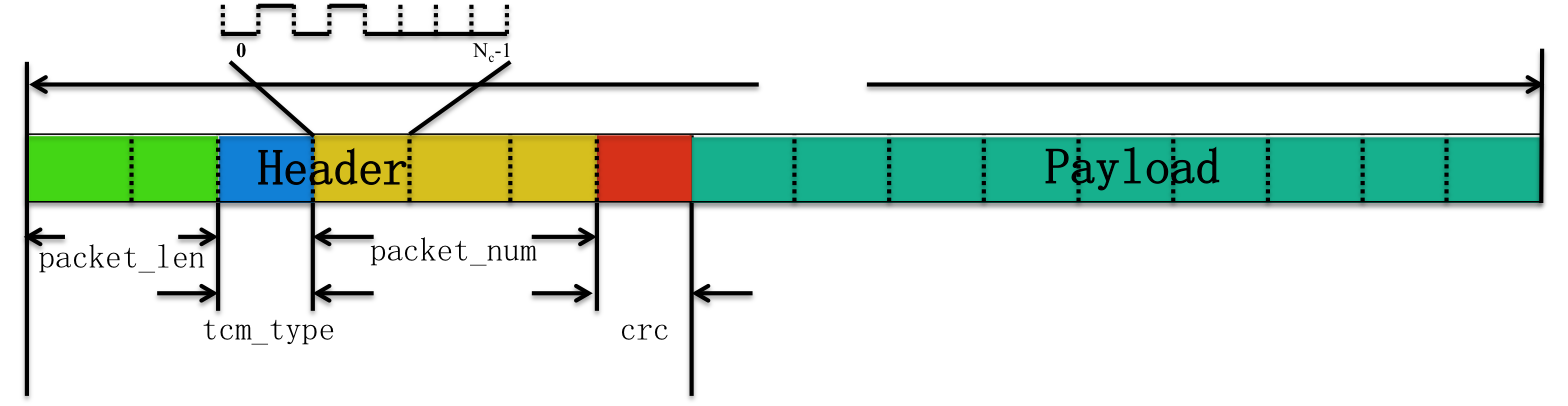
\includegraphics[width = 5in]{figure/data_frame.png}
	\caption{Data Frame}
	\label{fig:data_frame}
\end{figure}
\begin{figure}[ht]
	\centering
	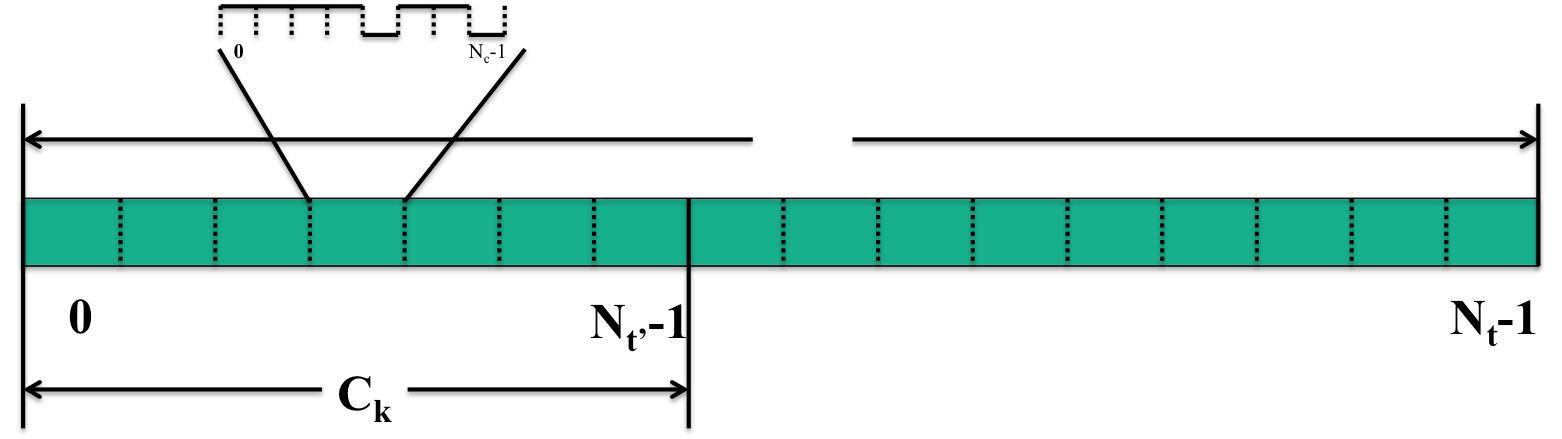
\includegraphics[width = 5in]{figure/training_frame.png}
	\caption{Training Frame}
	\label{fig:training_frame}
\end{figure}

In current version, because the number of binary bits for each Segment of the frame is set through ``python/cdma\_parameter.py'', the length for these part is 
\begin{table}[ht]
	\centering
	\caption{Length for Each Part of Frame}
	\label{tab:Length_for_each_part_of_frame}
	\begin{tabular}{ccc}
	\hline
		Frame Type 	& Segment Type 	& Segment Length\\ \hline
		Training 	& /		 		& 260			\\
		Data 		& packet length & 12 			\\
		Data 		& tcm type 		& 4 			\\
		Data 		& packet index 	& 16 			\\
		Data 		& header crc 	& 8 			\\ \hline
	\end{tabular}
\end{table}
% subsection packet_structure (end)

\subsection{Power Control} % (fold)
\label{sub:power_control}
As shown in the figure \ref{fig:diagram for Tx}, training sequence and data sequence are two separate branches. In reality, the power a transmitter could provide is certain, so before adding them up, the power arrangement should be considered. In ``python/cdma\_parameter.py'', variable ``training\_percent'' is to control the percentage of power used for Training sequence. 
% subsection power_control (end)

\subsection{Multi-Sampling and Pulse Shaping} % (fold)
\label{sub:multi_sampling}
Multi-Sampling is good for synchronization. In modern CDMA communication systems, like GPS, each chip will be sampled twice. Besides, we could not transmit digital signals directly, blocks like Root Raise-Cosine Filter will be added at the end of the block. The parameter set for RRCF is 
% subsection multi_sampling (end)
% section transmitter (end)




\bibliographystyle{plain}
\bibliography{bibliography.bib}

\end{document}
